\documentclass[main.tex]{subfiles}

\begin{document}
\begin{figure}[b]\centering
		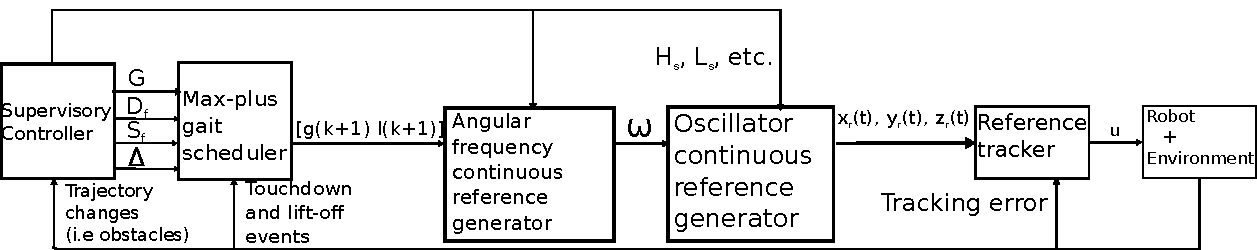
\includegraphics[width=0.95\textwidth]{ControlStrategy.pdf}
		\caption{Control strategy proposed. The supervisory controller based on the information obtained from the robot and the environment, provides the parameters to the scheduler in order to generate a proper gait given the current conditions. Out of the max-plus scheduler, the lift-off and touchdown times are passed to the angular frequency generator, which defines the angular frequency that it is used for the oscillator-based reference generator. The references are followed by a tracking controller.
			\label{fig:ControlStrat} }
\end{figure}
In this section the overview of the proposed strategy to control the locomotion pattern will be given. The overall control structured is depicted in Figure \ref{fig:ControlStrat}. 

The scheme is comprised by a) a supervisory control that makes use of sensory information to provide a set of parameters (both in time and space) in order to achieve coordinated locomotion, b) a max-plus gait scheduler, that realizes the gait according to the time parameters assigned by the supervisory controller, c) a continuous reference generator that decides the shape of the trajectory of each of the legs in space, using the spacial parameters given by the supervisory controller. The continuous trajectory generator is preceded by an angular frequency continuous reference generator, which translates the time differences obtained via the time scheduler into a continuous angular frequency reference for each of the legs in order to achieve the proper synchronism for the desired gait. At the end of the structure a reference tracking controller is in charge of following the generated trajectory and imposes the input for each of the legs onto the robot. 

There are three main feedback loops: one related to the reference tracking controller to correct the trajectory error, a second one related to the max-plus gait scheduler which detects the touchdown and lift-off events to update future timings in case of failure to reach or leave the ground, and the main feedback loop related to the supervisory controller which is in charge of modulating both the trajectory and time variables. In the following sections, each of the elements will be explained in more detail, except for the reference tracker and the robot plus environment blocks, which are not considered in this proposal.
\subsection{Supervisory controller}
The parameters given by the supervisory can be divided into two main groups: shape and time parameters. The shape parameters, determine the trajectory that each of the legs is going to follow, which in this case could be the step length $L_s$, step height $H_s$ and the oscillator function that determines the "primitive" shape that of the trajectory. The time parameters on the other hand, determine the speed and more importantly, the timed events between each of the legs in order to achieve a coordinated motion. These parameters are the duty factor $D_f$, the step frequency $S_f$, the gait pattern $G$ and the synchronization time vector $\Delta$. 

The gait pattern $G = \{L_{1,1},...,L_{1,j}\} \prec ... \prec \{L_{r,1},...,L_{r,j}\}$ represents the order in which groups of legs $L_j$, for $j = 1,...,n$ (n: number of legs), will move corresponding to an specific pattern. For example for a quadruped diagonal trotting gait, with the legs defined as in Table \ref{Table:LegIndexes},one would write:
\begin{table}[t]
\centering
\caption{Definition of leg indexes.}
\label{Table:LegIndexes}
\begin{tabular}{|l|l|l|}
\hline
Leg         & Leg index convention & Leg index number \\ \hline
Left front  & LF                   & 1                \\ \hline
Right front & RF                   & 2                \\ \hline
Left hind   & LH                   & 3                \\ \hline
Right hind  & RH                   & 4                \\ \hline
\end{tabular}
\end{table}
\begin{equation}
G = \{1,4\}\prec\{2,3\},
\end{equation}
likewise, a gait where only one leg at a time is in swing phase would be described as:
\begin{equation}
G = \{1\}\prec\{2\}\prec\{3\}\prec\{4\}.
\end{equation}
The vector $\Delta$ is comprised by the time differences between each of the leg groups in $G$. These time differences are chosen by the supervisory control in order to achieve certain gait pattern. For example, for a trotting diagonal gait, $\Delta$ would be constructed by two elements:
\begin{equation}
\Delta = \begin{bmatrix} \Delta_1 & \Delta_2
\end{bmatrix},
\end{equation}
where $\Delta_1$ and $\Delta_2$ are the time differences between the first and the second leg group and the one corresponding from the second to the first, respectively, as depicted on Figure \ref{fig:TrotTime}. These values represent the time each leg has to wait (or anticipate) to reach its lift-off event. If the leg needs to wait for an event, $\Delta_i$ would take a positive value, on the other hand if the leg needs to anticipate its lift-off time, $\Delta_i$ would assume a negative value.
\begin{figure}[t]\centering
		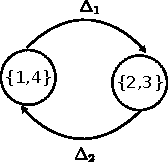
\includegraphics[width=0.25\textwidth]{TrotTime.pdf}
		\caption{Example of the switch between leg groups for a diagonal trotting gait. The time between the first group and the second group is $\Delta_1$ and the time from the second group to the first one is $\Delta_2$.
			\label{fig:TrotTime} }
\end{figure}

The supervisory controller can use this set of time parameters to actively change the locomotion pattern depending on the situation that the robot is facing. Furthermore, these synchronization parameters in $\Delta$ can be designed according to a cost function related to an optimization problem, similar to what is done in \cite{Park2015} to choose the phase differences between legs. The advantage of this approach, is that this could potentially be modified online, since all the event dynamics are linear (this is, in the max-plus sense, and explained in the next section), would not require high amounts of computational time. 

It has to be noted though, that the task of guaranteeing that "smooth" transitions between gaits is still open, since sudden and very diverse changes may cause odd and "limping" movements on the robot. One approach that could be considered is the one taken in \cite{Park2015,Asif2011}, where either a linear function was designed in order to achieve the transition in a smooth manner, or an optimization routine could be established as well in order to select a proper transition function between gait parameters from trot to gallop. In addition, to achieve a feasible gait pattern and to keep a desired duty factor $D_f$ and step frequency $S_f$, there are some constraints regarding the selection of $\Delta$. For example, the total sum of each of the elements is subject to the following equation:
\begin{equation}
\sum_{i = 1}^{n} \tau_i \leq \frac{1}{S_f}(1 - j(1 - D_f)) \textmd{ with n: number of leg groups}.
\end{equation}
This expression constraints the total sum of time differences, since in order to keep a duty factor and a step frequency during the whole cycle, the sum of time differences cannot be greater than the step period ($\frac{1}{S_f}$)  minus the time each legs spends in swing phase, multiplied by the number of legs $j$. There are also other limitations that need to be studied, since it has been noticed in simulation that there are also changes in the gait sequence related to the minimum value that each $\Delta_i$ can assume depending on the chosen duty factor. This is also a task to be tackled in the future.
\subsection{Max-plus gait scheduler}\label{section:MaxPlus}
Using the parameters given by the supervisory controller block, max-plus gait scheduler manages the time sequence for each of the legs in order to achieve the desired coordination. What comes out of the max-plus gait scheduler block are the touchdown and lift-off time events for each of the legs, which are obtained in a systematic manner making use only of the user input values given by the supervisory controller. Despite its simplicity, there are some advantages of using this type of systems to achieve coordination, since it represents a systematic method to assign the moments when each leg is going to move. Moreover, properties of transition and stability of the gait cycle can be analysed using max-plus linear systems theory.

\paragraph{Basics of max-plus algebra.}As an initial step, the basic concepts of this so-called "tropical algebra" are explained based on \cite{Schutter2008}. Consider the following algebra:
\begin{equation}
	(\Re_{max}, \oplus, \otimes, \varepsilon, e),
\end{equation}
where:
\begin{align}
	\Re_{max} &:= \Re \cup \{-\infty\}, \nonumber\\
	x \oplus y &:= max(x,y), \nonumber\\
	x \otimes y &:= x + y, \nonumber\\
	\varepsilon &:= -\infty, \nonumber\\
	e &:= 0. \nonumber
\end{align}
In place, this algebra is defined by the set of real numbers including the negative infinity; the two binary operations: the maximum of two numbers and the addition; the absorbing element $\varepsilon$ given by $-\infty$ and the identity element given by $0$. Subsequently, max-plus algebra can be extended to matrices defined by the following structure:
\begin{equation}
	(\Re_{max}^{n\times m}, \oplus, \otimes,\mathcal{E}, E),
\end{equation}
with:
\begin{align}
	[A \oplus B]_{ij} &= a_{ij} \oplus b_{ij} := \max(a_{ij},b_{ij}), \nonumber \\
	[A \otimes C]_{ij} &= \underset{k=1}{\overset{m}{\mathlarger{\mathlarger\oplus}}}a_{ik} \otimes c_{kj} := \max\limits_{k=1,...,m}(a_{ik} + c_{kj}), \nonumber 
\end{align}
where $A,B \in \Re_{max}^{n\times m}$, $C \in \Re_{max}^{m\times p}$, and the $i,j$ element of $A$ is denoted by $a_{ij} = [A]_{ij}$, and identity and zero matrices defined by:
\begin{align}
	[\mathcal{E}]_{ij} &= \varepsilon, \nonumber \\
	[E]_{ij} &= \begin{cases}
		e, & \text{if } i =j \\
		\varepsilon,& \text{otherwise.}
	\end{cases} \nonumber
\end{align}
Powers of matrices can also be defined as:
\begin{equation}
	D^{\otimes k} :=\underbrace{ D \otimes D \otimes... \otimes D}_\text{k-times}.
\end{equation}
The max-plus algebra structure corresponds to a commutative idempotent semiring. 

\paragraph{Max-plus algebra applied to legged locomotion.}Max-plus linear systems have been used to model legged locomotion, abstracting the continuous-time motion of the legs into discrete event cycles \cite{Lopes2009}. Let $g_i(k)$ be the time instant when leg $i$ touches the ground (touchdown time at time instant $k$) and $l_i(k)$ the time instant when it lifts-off from the ground (lift-off time at time instant $k$). We can describe the touchdown time as a function of the lift-off time plus the time instant that the leg stays in swing phase, i.e.:
\begin{equation}
g_i(k+1) = l_i(k+1) + \frac{1}{S_f}(1 - D_f).
\end{equation}
Furthermore, the lift-off time instant can be defined as the previous touchdown time plus the time that the leg remains in stance phase,i.e.:
\begin{equation}
l_i(k+1) = g_i(k) + \frac{1}{S_f}D_f.
\end{equation}
These two equations can be used iteratively to generate the movement of a single leg. In the case where several leg cycles want to be represented, we can define the following state vector:
\begin{equation}
X(k) = \begin{bmatrix}
\smash{\underbrace{\begin{matrix}g_1(k) & ... & g_n(k)\end{matrix}}_{g(k)}} & \smash{\underbrace{\begin{matrix}
l_1(k) & ... & l_n(k)
\end{matrix}}_{l(k)}}
\end{bmatrix},\label{eq:StateVector}
\end{equation}

\vspace{0.3cm}
with $n$ being the number of legs. By doing this, the leg cycles can be written in the following max-plus algebra linear system:
\begin{equation}
\begin{bmatrix}
g(k + 1) \\
l(k + 1)
\end{bmatrix} =
\begin{bmatrix}[c|c]
\mathcal{E} & \frac{1}{S_f}(1 - D_f) \otimes E \\ \hline
\mathcal{E} & \mathcal{E}
\end{bmatrix} \otimes \begin{bmatrix}
g(k + 1) \\
l(k + 1)
\end{bmatrix} \oplus \begin{bmatrix}[c|c]
\mathcal{E} & \mathcal{E} \\ \hline
\frac{1}{S_f}D_f \otimes E & \mathcal{E}
\end{bmatrix} \otimes \begin{bmatrix}
g(k) \\
l(k)
\end{bmatrix}.
\end{equation}
where $\mathcal{E}$ and $E$ are the identity and zero matrices as defined previously. If one wants to coordinate legs $i$ and $j$, so that leg $i$ lifts-off $\Delta_i$ seconds before (or after, if $\Delta_i$ is negative) after leg $j$ has touched the ground. This can be expressed in the following relation:
\begin{equation}
l_i(k+1) = \max (g_i(k) + \frac{1}{S_f}D_f, g_j (k) + \Delta_i),
\end{equation} 
which can be written in max-plus algebra as:
\begin{equation}
l_i(k+1) = \begin{bmatrix}
\frac{1}{S_f}D_f & \Delta_i
\end{bmatrix} \otimes \begin{bmatrix}
g_i(k) \\
g_j(k)
\end{bmatrix}.\label{eq:SynchOneLeg}
\end{equation}
If coordination wants to be achieved for group of legs, a relation between the next lift-off time of a leg with the touchdown times of the other legs can be enforced, as done in the case of Equation \eqref{eq:SynchOneLeg}. This can be written as a max-plus linear system using the state vector definition of Equation \eqref{eq:StateVector} in the following way:
\begin{equation}
\begin{bmatrix}
g(k + 1) \\
l(k + 1)
\end{bmatrix} =
\begin{bmatrix}[c|c]
\mathcal{E} & \frac{1}{S_f}(1 - D_f) \otimes E \\ \hline
P & \mathcal{E}
\end{bmatrix} \otimes \begin{bmatrix}
g(k + 1) \\
l(k + 1)
\end{bmatrix} \oplus \begin{bmatrix}[c|c]
\mathcal{E} & \mathcal{E} \\ \hline
\frac{1}{S_f}D_f \otimes E \oplus Q& \mathcal{E}
\end{bmatrix} \otimes \begin{bmatrix}
g(k) \\
l(k)
\end{bmatrix},\label{eq:MaxPlusLinear}
\end{equation}  
where $P$ and $Q$ matrices represent matrices of time differences according to the gait pattern $G$ and the synchronization vector $\Delta$. This can be written in a more compact way as:
\begin{equation*}
x(k+1) = R \otimes x(k+1) \oplus H \otimes x(k)
\end{equation*}
Up to this point it is not clear if Equation \eqref{eq:MaxPlusLinear} can be solved explicitly (find $x(k+1)$ as a function dependent on $x(k)$). The solution to this problem is given in \cite{Lopes2009,Lopes2010} and provides the following equation:
\begin{equation*}
x(k+1) = R^* \otimes H \otimes x(k),
\end{equation*}
and the existence of the matrix $R^*$ is proven due to the fact that $P$ is a nilpotent matrix. In fact, in \cite{Lopes2009}, using the previously proposed parametrization of the gait space given by $G$, an explicit and systematic way to compute matrices $Q$ and $P$ was derived. A minor difference of the approach taken in this document is that, in the case of \cite{Lopes2009} all $\Delta_i$ values in the vector $\Delta$ were the same, whereas in here we try to give more versatility to possible number of gaits by giving different value to each $\Delta_i$.
\paragraph{Property analysis of the gait cycle using max-plus algebra theory.}As mentioned before, one of the advantages of using max-plus algebra systems is the possibility to study the properties of the cycle. 
If the matrix $A = R^*H$, one could find the max-plus eigenvalues and eigenvectors. It has been shown that matrix $A$ has a unique eigenvalue, and it represents the total cycle time. On the other hand, the eigenvector is a representation of the steady state behaviour of the system. Another property investigated in previous studies is the so-called, coupling time refers to the number of finite steps that it takes for a system to reach a steady-state regime. This represents the transient behaviour, for example, while switching from one gait to another, it can be thought of in a similar way as the settling time for continuous-time systems. It has been proven that for a class of max-plus linear system the coupling time, denoted by $k_0$, is equal to 2. This means that it takes at most two cycle steps to reach max-plus steady-state when there is a perturbation.

This properties, have been used to provide ways for optimal gait switching, and to estimate the forward velocity of the robot in \cite{Lopes2009}.

It has to be noted though, that some of these properties have been found to locomotion under very specific conditions (i.e. $\Delta_1=...=\Delta_i$, non-ballistic gaits with $\Delta_i > 0$, among others). Despite this fact, most of the research leaves as further work to investigate if this properties are valid for a wider range of locomotion conditions.
\subsection{Angular frequency continuous reference generator}
\begin{figure}[b]\centering
		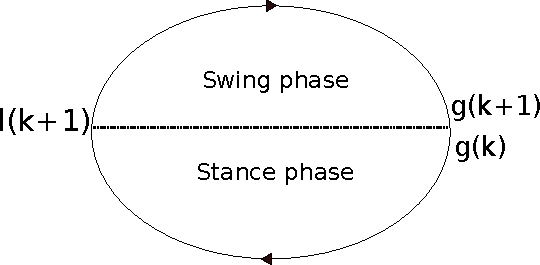
\includegraphics[width=0.4\textwidth]{Phases.pdf}
		\caption{Phases of movement for an elliptical trajectory.
			\label{fig:Phases} }
\end{figure}
The angular frequency reference generator constitutes a key element in order to implement the timed events given by the max-plus scheduler into a continuous-time framework. Initially the trajectory is divided in two sections corresponding to the swing and stance phases, each with specific periods $Ti_{st}$ and $Ti_{sw}$, respectively, and they are defined as follows:
\begin{align}
Ti_{st} &= l_i(k+1) - g_i(k) \\
Ti_{sw} &= g_i(k+1) - l_i(k+1),
\end{align}
where $l_i(k)$ and $g_i(k)$ are the lift-off and touchdown times leg $i$ at time event $k$. Figure \ref{fig:Phases} shows a drawing of the distinction between the two phases and the location where the touchdown and lift-off events take place. Using these two periods, we define an average angular frequency $\omega$ for the swing and stance phases. This angular frequency should be defined according to the trajectory that wants to be achieved, and it is defined as follows:
\begin{equation}
\bar{\omega} = \begin{cases}
\frac{\pi}{Ti_{st}} \textbf{ for } t \in [g_i(k),l_i(k+1)] \\
\frac{\pi}{Ti_{sw}} \textbf{ for } t \in (l_i(k+1),g_i(k+1)] 
\end{cases}\label{eq:angularfreq}
\end{equation}
The average angular frequency $\bar{\omega}$ is a parameter which ensures that the swing and stance phases will be reached at the appropriate time events in order to keep the synchronism of the gait. In this report, the angular frequency is just defined as a constant value equal to the average angular frequency in \ref{eq:angularfreq}. It would be desirable though, that this angular frequency was designed as a smooth transitioning function that would allow to keep the average along both swing and stance phase trajectories, thus complying with the following condition:
\begin{equation}
\frac{1}{Ti_{p}}\int^{Ti_{p}} \omega dt = \bar{\omega} \textbf{ for } p = st,sw.\label{eq:angularfrequencycondition}
\end{equation} 
Furthermore, it is also preferred that the movements during swing phase could be modulated, for example having faster motions in the beginning of the phase while slowing down towards the end. This situation could be approached in two different ways. The first one could be proposing another time event at the "highest" point of the ellipse, so one could have different functions for the angular frequency for the two halves of the swing phase. The second approach would be designing a profile function for $\omega$ in such a way that it complies with the condition given in \ref{eq:angularfrequencycondition}. This second approach seems more appealing since it would imply not restating the max-plus algebra system (since the equations in Section \ref{section:MaxPlus} would no longer apply), and could potentially provide more freedom on how the movement in both phases is achieved, given a suitable design for the function of $\omega$ (i.e., via the solution of an optimization problem).
\subsection{Oscillator continuous reference generator}
The oscillator continuous reference generator corresponds to the equations given in \cite{Barasuol2013} and a "squared" version of these equations used during simulation in this report. The main difference in this report lies on the fact that the coupling matrix used for synchrony is neglected here, since its function is being fulfilled by the max-plus algebra scheduler and the angular frequency continuous reference generator. The supervisory controller is in charge of defining the main shape parameters of the trajectory such as step length $L_s$ and step height $H_s$. In this document we comprised these parameters in the variables $a$ and $b$. The equations used for the elliptical case are given by:
\begin{align}
x = \alpha (1 - \frac{x^2}{a^2} - \frac{z^2}{b^2})x + \frac{\omega a}{b}z \\
z = \beta (1 - \frac{x^2}{a^2} - \frac{z^2}{b^2})z - \frac{\omega b}{a}x,
\end{align}
and in the case of the "squared" oscillator are given by:
\begin{align}
x = \alpha (1 - \frac{x^4}{a^4} - \frac{z^4}{b^4})x + \frac{1.18\omega a}{b^3}z^3 \\
z = \beta (1 - \frac{x^4}{a^4} - \frac{z^4}{b^4})z - \frac{1.18\omega b}{a^3}x^3.
\end{align}
\subsection{Simulations}
Using the previous scheme a simulation was performed consisting on the implementation of 2 different gaits, each of those with 2 variations where the gait parameters $D_f$ and $\Delta$ are changed. These 4 variations, switch between each other at specific times throughout the process. The gait patterns are summarized in Table \ref{Table:GaitParameters}.
\begin{table}[b]
\centering
\caption{Gait parameters used in simulation}
\label{Table:GaitParameters}
\begin{tabular}{|l|l|l|l|l|}
\hline
       & $G$                                   & $D_f$ & $S_f[\frac{1}{s}]$ & $\Delta[s]$                                                 \\ \hline
Gait 1 & $\{1,4\}\prec\{2,3\}$                 & 0.8  & 0.5        & $\begin{bmatrix} 0.24 & 0.48\end{bmatrix}$               \\ \hline
Gait 2 & $\{1,4\}\prec\{2,3\}$                 & 0.2  & 0.5        & $\begin{bmatrix} -0.1 &-1.2\end{bmatrix}$                \\ \hline
Gait 3 & $\{1\}\prec\{2\}\prec\{3\}\prec\{4\}$ & 0.8  & 0.5        & $\begin{bmatrix} 0.1 & 0.1 & 0.1 & 0.1\end{bmatrix}$     \\ \hline
Gait 4 & $\{1\}\prec\{2\}\prec\{3\}\prec\{4\}$ & 0.2  & 0.5        & $\begin{bmatrix} -1.5 & -1.9 & -1.1 & -1.1\end{bmatrix}$ \\ \hline
\end{tabular}
\end{table}
The gait parameters are changed from Gait 1 to Gait 4 every 10 seconds. The purpose of this is first, prove that the proposed strategy is able to coordinate legs while providing a desired trajectory given by the oscillator equations, and second visualize the effects of changing gait parameters while the robot is moving. 

Figure \ref{fig:SyncPlot} shows the pattern generated by the current strategy. In this plot it can be seen that regarding synchronization, the strategy is able to generate various types of gaits, of course it remains to be proven if these gaits are feasible, since up to this point we are not considering the dynamics of the robot itself. Furthermore, depending on how aggressive" the change of gait is and the difference between duty factors, the convergence to the new gait takes different times. This is a problem because if fast reactions are needed, there must be a reliable way to know how much will the gait switch will take. I personally believe that, if the change of paramaters is designed having a smooth transition in between gaits it is possibly to know the time that it will take to converge from one gait to the other, and furthermore, how far ahead one has to plan the changes on the gait parameters.
\begin{figure}[t]\centering
		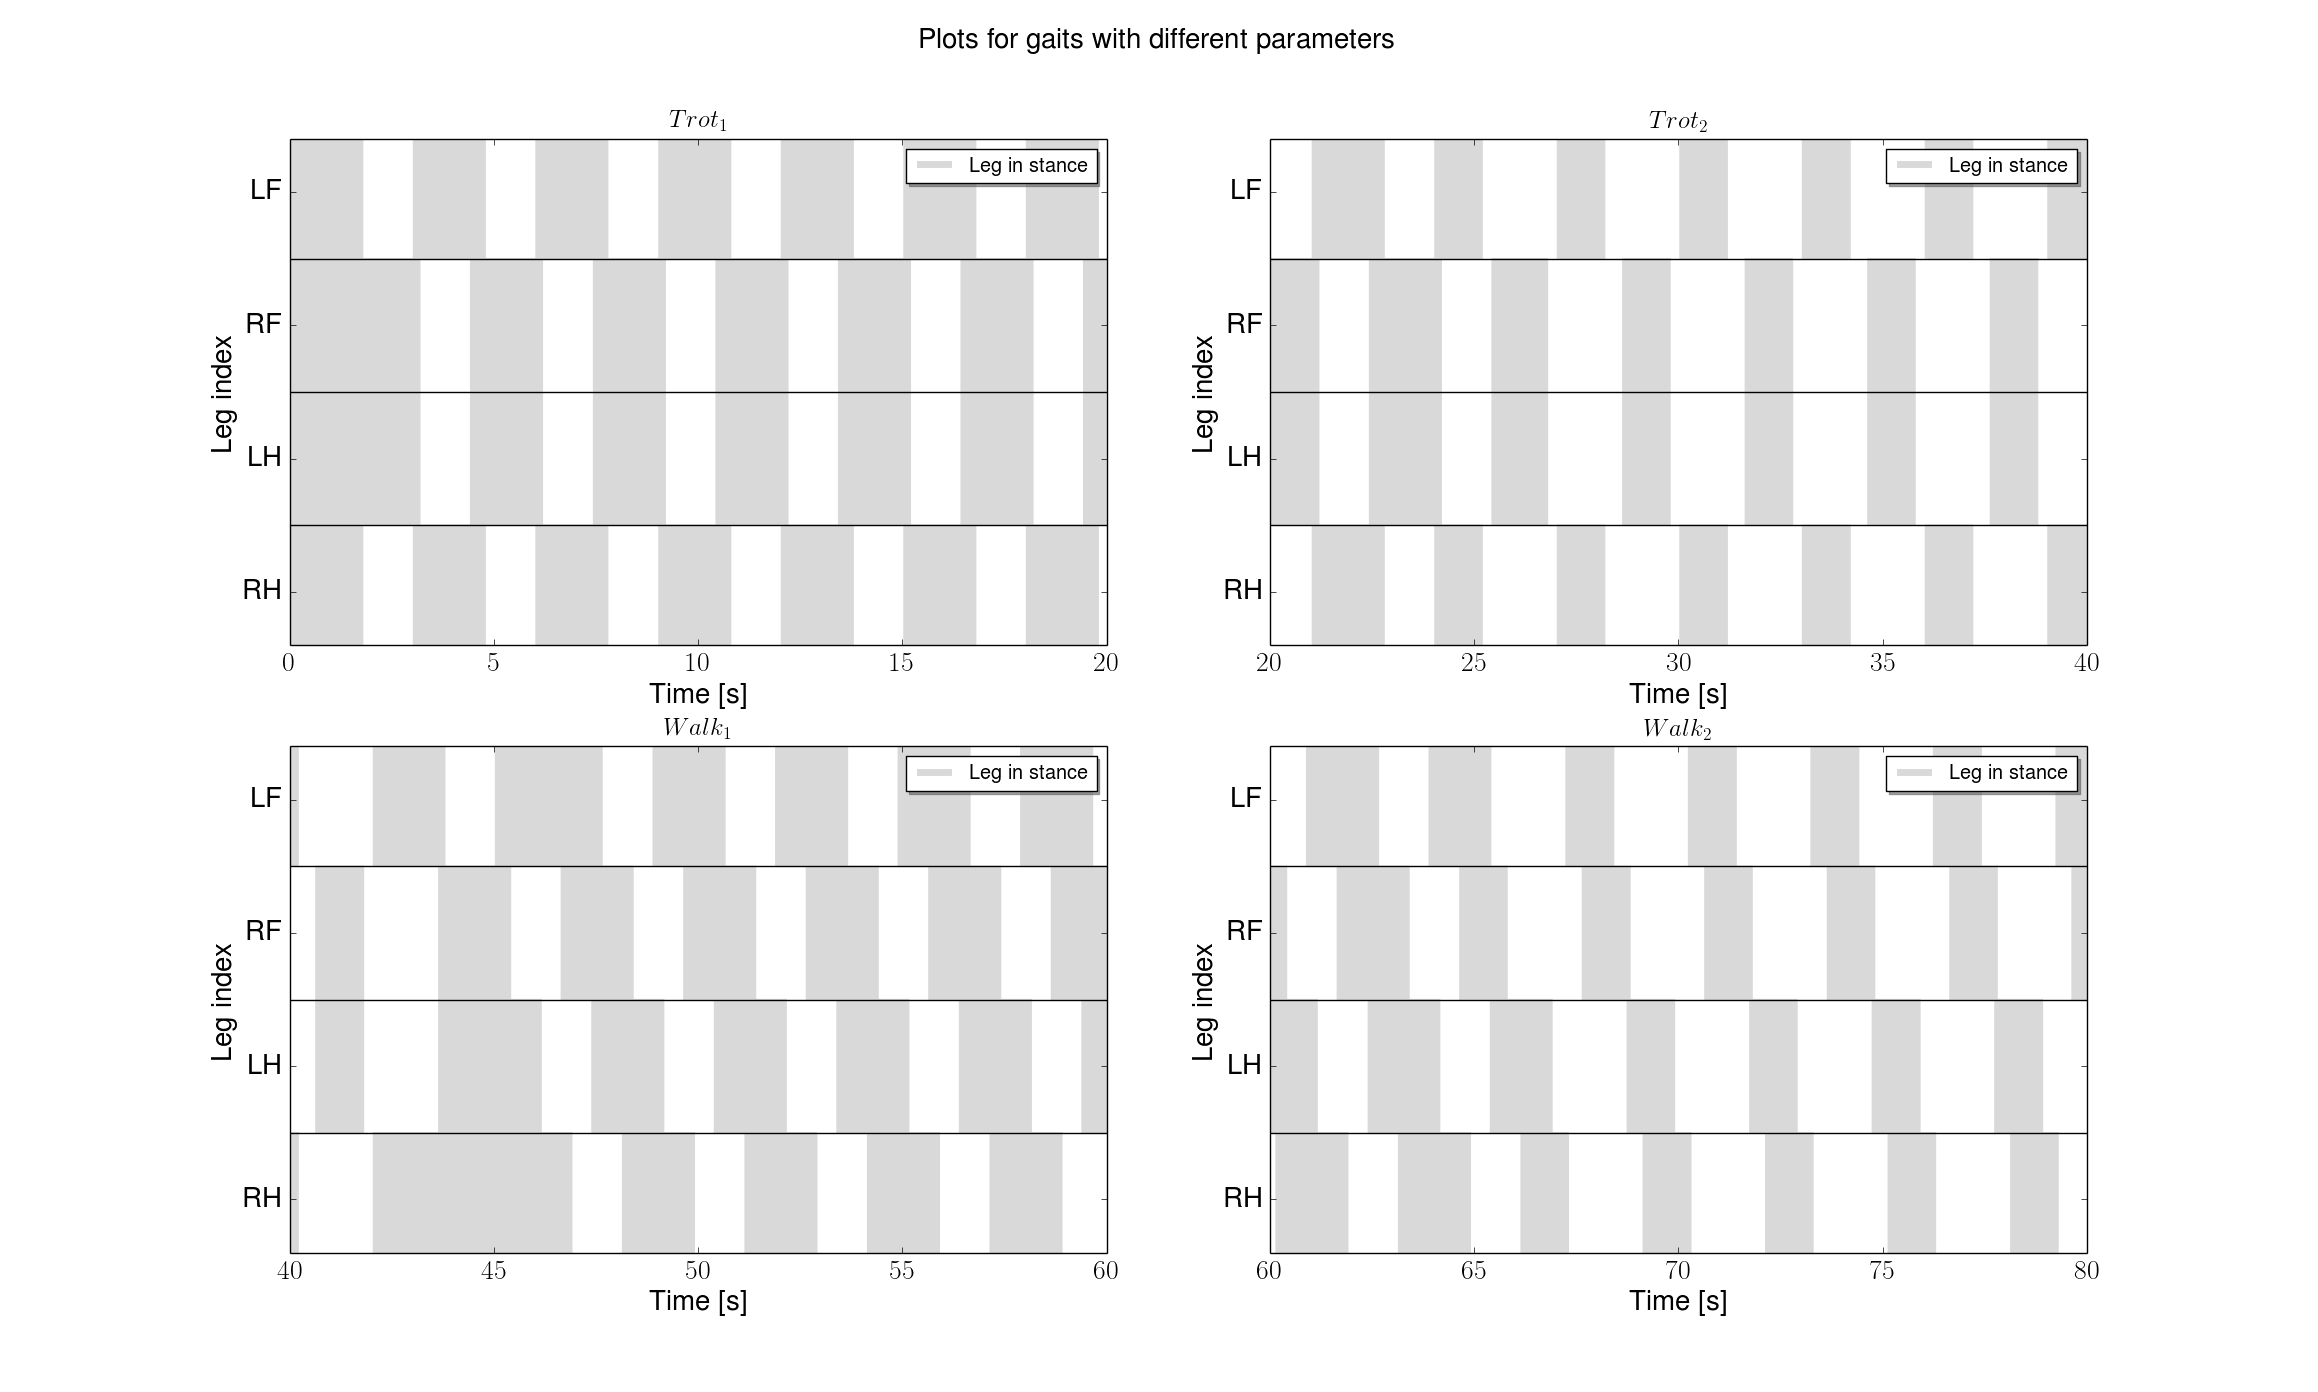
\includegraphics[width=0.8\textwidth]{SyncPlot.png}
		\caption{Pattern plot corresponding to the simulation. Gray blocks represent that the leg is on the ground, while white space represents that the leg is not touching the ground. The blue dashed lines indicate the moments when a gait change is decided.
			\label{fig:SyncPlot} }
\end{figure}

Considering the trajectory to be followed, in both cases (elliptical and squared) the proposed method was able to follow the reference if proper values of $\alpha$ and $\beta$ are chosen (if these are not large enough the convergence properties of the oscillator may cause phase differences with respect to the desired trajectories). Figure \ref{fig:HeightTime} shows the evolution of reference coordinate $z$ with respect to time from 5 to 25 seconds (the result is the same for the rest of the trajectory). It can be seen in the plot that the leg touches and leaves the ground at the specific times designated by the max-plus algebra scheduler (denoted by the dashed lines). Nevertheless, it still remains the task to deal first with disturbances such as tracking errors or the case were a touchdown or lift-off event is not reached (which is tackled by updating the max-plus algebra time scheduler).
\begin{figure}[t]\centering
		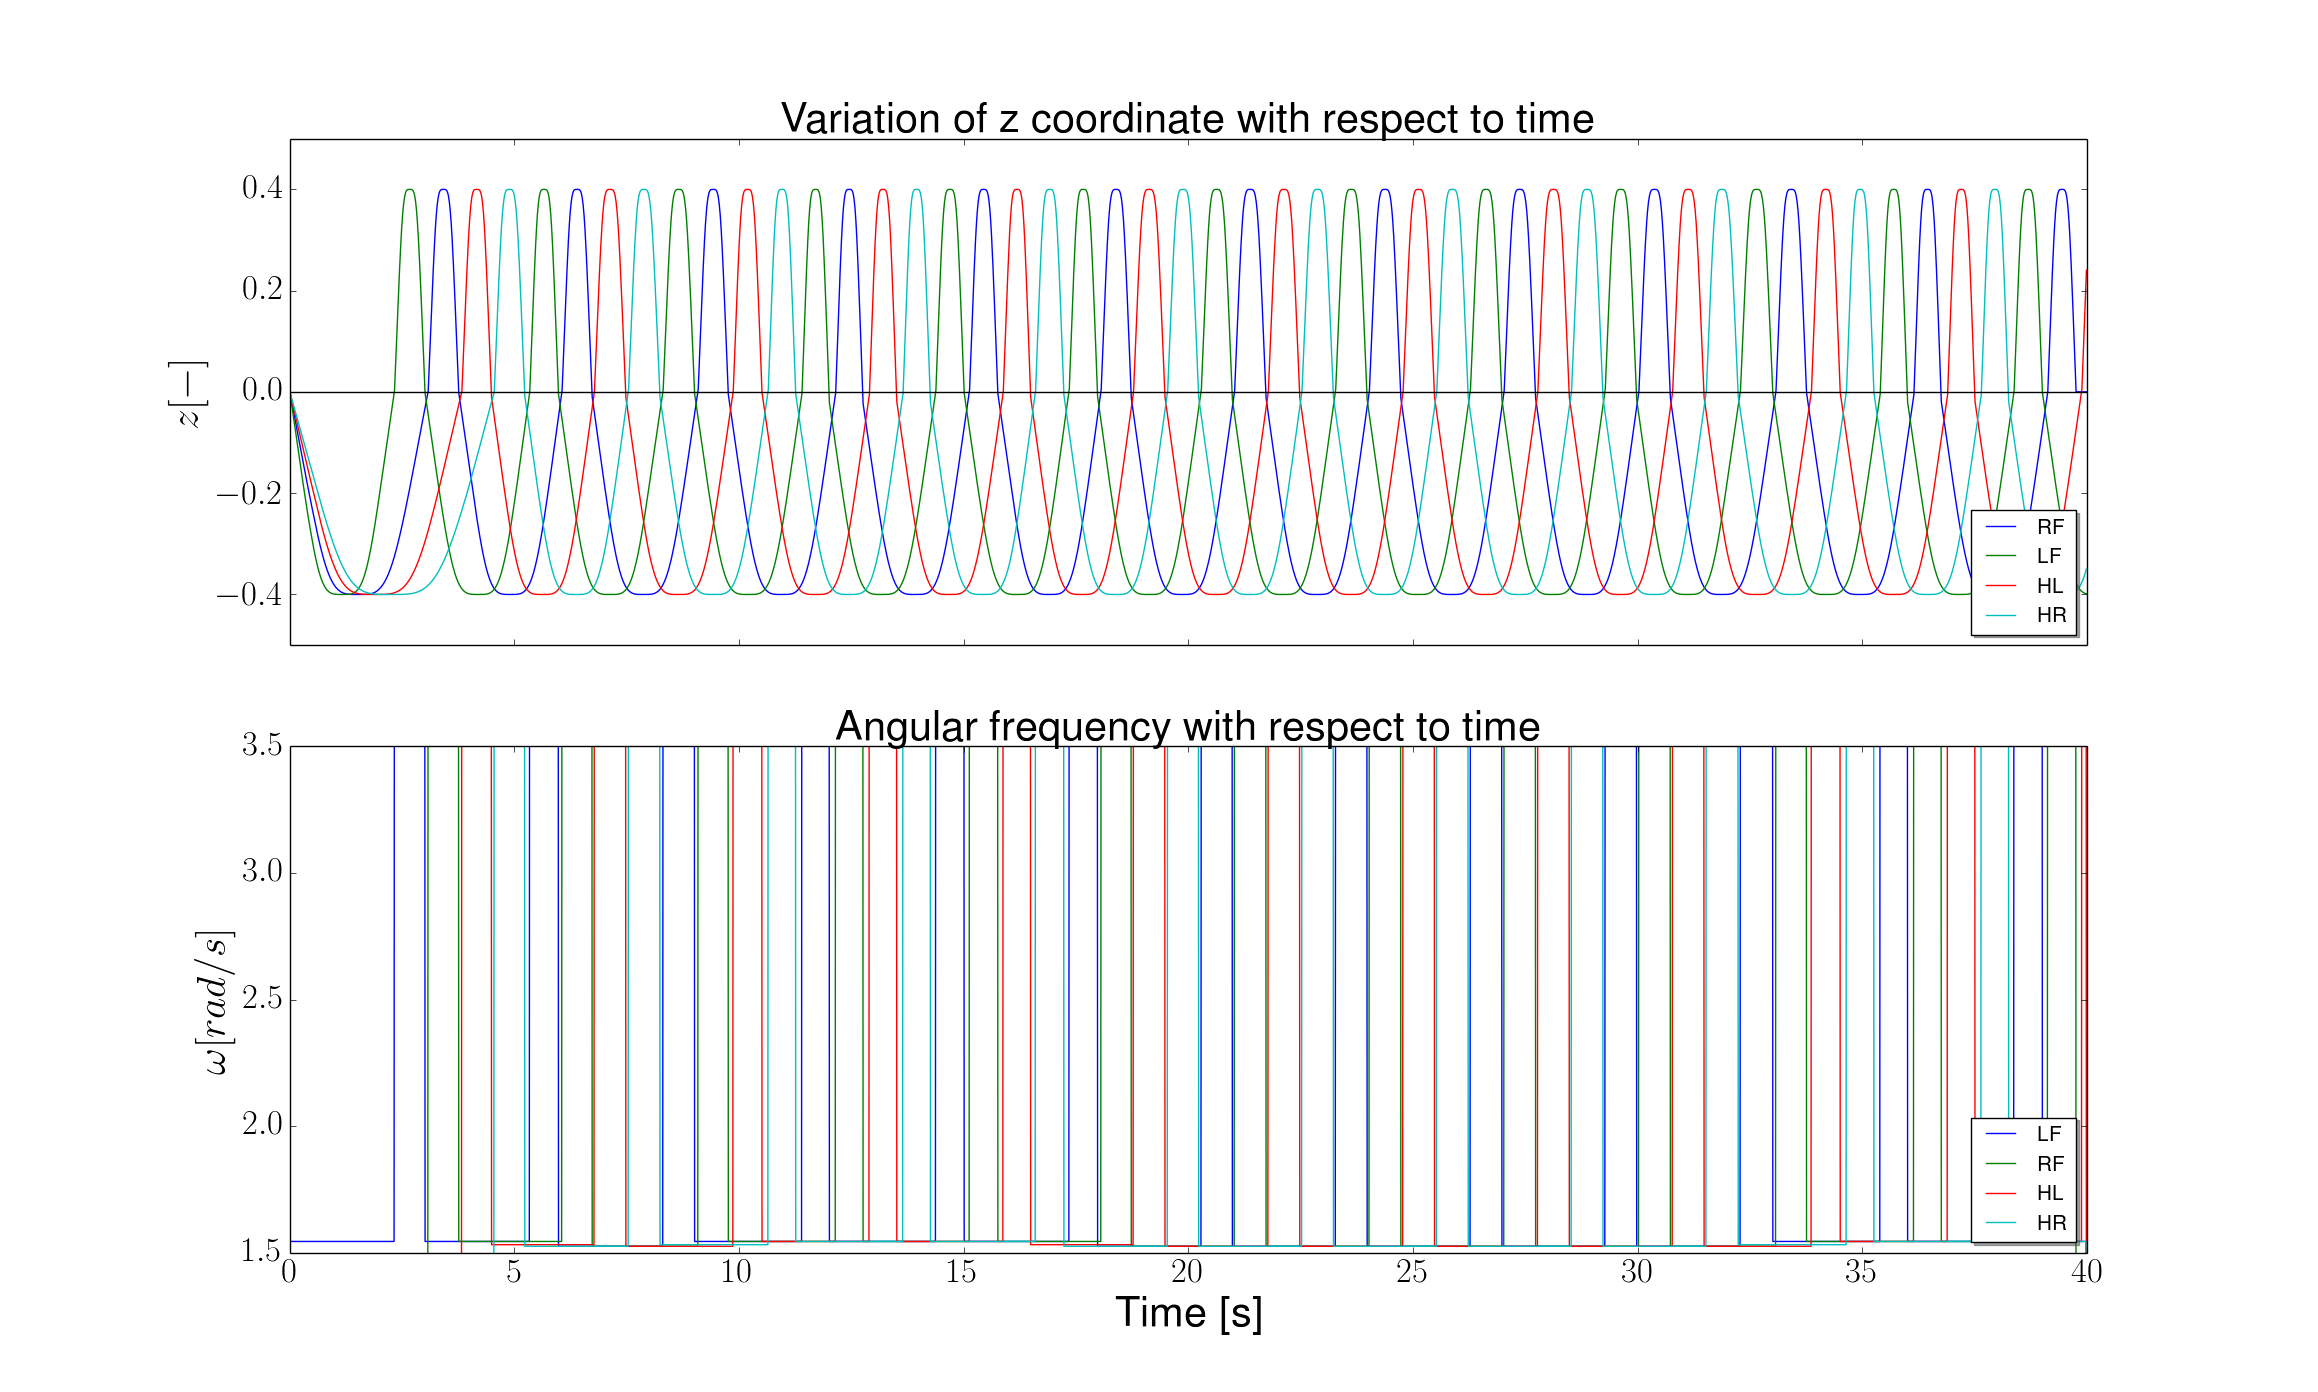
\includegraphics[width=0.8\textwidth]{HeightTime.png}
		\caption{Plot showing the evolution of coordinate $z$ with respect to time from 5 to 25 seconds. The dashed lines indicate the touchdown and lift-off times (i.e. the moments were the angular frequency is changed).
			\label{fig:HeightTime} }
\end{figure}

Finally, a plot of the angular frequency $\omega$ with respect to time is shown in Figure \ref{fig:AngularFrequency}. This plot shows that the angular frequency changes its constant value from swing to stance phase depending on the references given by the max-plus algebra time scheduler. The main issue with keeping constant the value of the angular frequency, is that at the beginning and ending of the "faster" phases(the swing and stance could last less or longer depending on the duty factor), the legs execute really aggressive movements. It is obvious that this could be improved if a function that respects the condition given in Equation \ref{eq:angularfrequencycondition} is designed to avoid this aggressive changes in angular frequency, providing more freedom to modulate de behaviour.
\begin{figure}[t]\centering
		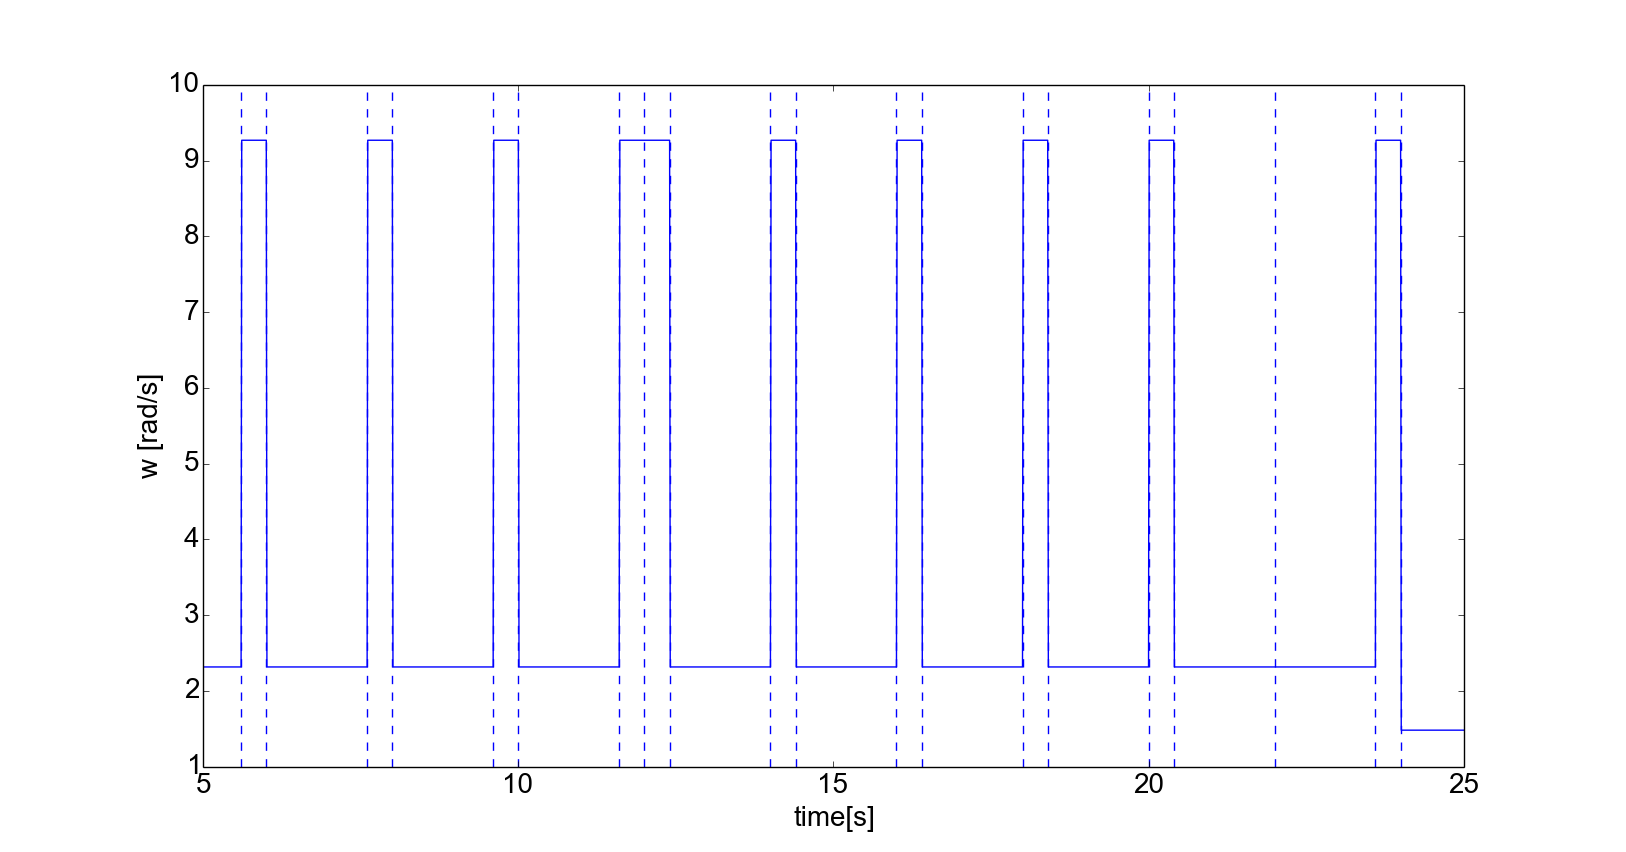
\includegraphics[width=0.8\textwidth]{AngularFrequency.png}
		\caption{Angular frequency with respect to time. Dashed lines indicate touchdown and lift-off times.
			\label{fig:AngularFrequency} }
\end{figure}

\end{document}